\section{Experiments}
\label{sec:exp}
In this section, we first describe the dataset used in our paper. We then introduce all baselines, evaluation metric, and setting. Finally, we present our research questions and results.

\subsection{Dataset}
\label{sec:dataset}
\cmt{TODO: add the information about the dataset}

\subsection{Baseline}
\label{sec:baseline}
We compared DeepJIT with two other state-of-the-art baselines in the \emph{Just-In-Time} (JIT) defect prediction:
\begin{itemize}
\item JIT: The method for identifying fix-inducing code changes was proposed by McIntosh and Kamei~\cite{mcintosh2018fix}. The method used a nonlinear variant of multiple regression modeling~\cite{fox1997applied} to build a classification model for automatically identifying defects in commits. The set of code features, using six families of code change properties, are primarily derived from prior studies~\cite{Kamei:2013:LES, Kim:2008:CSC, Kononenko:2015, Mockus2000}. These properties are: the magnitude of change, the dispersion of the changes, the defect proneness of prior changes, the experience of the author, the code reviewers, and the degree of participation in the code review. 
\item DBN-JIT: The method adopted Deep Belief Network (DBN)~\cite{hinton2006reducing}, one of the state-of-the-art deep learning approaches, to generate a more expressive feature set from the initial feature set. The generated feature set,  
\end{itemize}

\subsection{Training and hyperparameters}
\label{sec:training_parameters}
For the size of the convolutional filters, we choose 64. The size of DeepJIT's fully-connected layer described in Section~\ref{sec:ftr_combine} is set to 512. The word vectors dimension of the commit message ($d_m$) and code changes ($d_c$) are set to 64. We train DeepJIT using Adam~\cite{kingma2014adam} with shuffled mini-batches.  The batch size is set to 32. We train DeepJIT for 100 epochs. We also apply the early stopping strategy~\cite{prechelt1998automatic, caruana2001overfitting} to avoid overfitting problem during the training process. Typically, we stop the training if the value of the objective function (see Equation~\ref{eq:cost}) has been no update in the last 5 epochs. All these hyperparameters in our paper are widely used in the deep learning community~\cite{severyn2015learning, huo2016learning, huo2017enhancing, hinton2012improving}. 
 

\subsection{Evaluation Metric and Setting}
\label{sec:metric_setting}

\subsection{Research Questions and Results}
\label{sec:rq_results}

\noindent \textbf{RQ1: How effective is our proposed deep learning model compared to the state-of-the-art baseline?}

\begin{figure}
\center
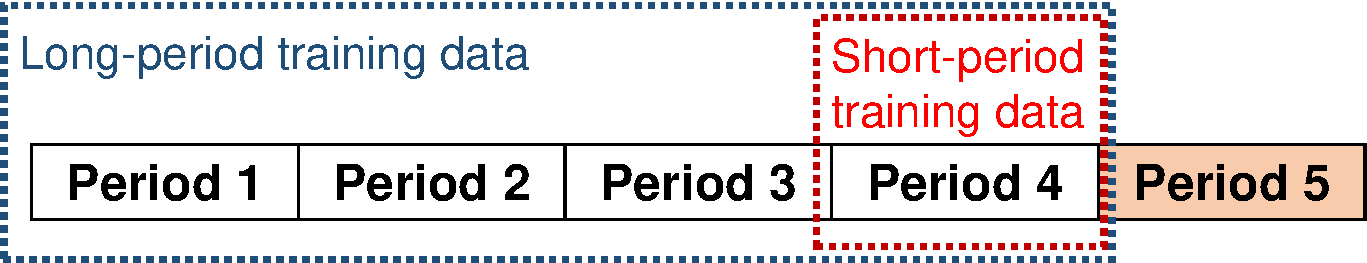
\includegraphics[scale=0.36]{figs/split.pdf}
\caption{An example of choosing the data for training proposed model. The last period will be used as testing data.}
\label{fig:splitting}
\end{figure}

\begin{table*}[t!]
  \centering
  \caption{The AUC results of DeepJIT vs. with other baselines in three settings: short-period, long-period, and random}
    \begin{tabular}{|l|c|c|c|c|c|c|}
    \hline
    \multirow{2}[4]{*}{} & \multicolumn{3}{c|}{QT} & \multicolumn{3}{c|}{OPENSTACK} \\
\cline{2-7}          & \multicolumn{1}{l|}{Short-Period} & \multicolumn{1}{l|}{Long-period} & \multicolumn{1}{l|}{Random} & \multicolumn{1}{l|}{Short-Period} & \multicolumn{1}{l|}{Long-period} & \multicolumn{1}{l|}{Random} \\
    \hline
    \hline
    JIT   & 0.703 & 0.702 & 0.701 & 0.711 & 0.706 & 0.691 \\
    \hline
    DBNJIT & 0.714 & 0.708 & 0.705 & 0.716 & 0.712 & 0.694 \\
    \hline
    DeepJIT & \textbf{0.764} & \textbf{0.765} & \textbf{0.768} & \textbf{0.781} & \textbf{0.771} & \textbf{0.751} \\
    \hline
    \end{tabular}%
  \label{tab:results}%
\end{table*}%

\noindent \textbf{RQ2: Does the proposed model benefit both commit message and the code changes?}

\begin{table*}[t!]
  \centering
  \caption{Contribution of feature components in DeepJIT}
    \begin{tabular}{|l|c|c|c|c|c|c|}
    \hline
    \multirow{2}[4]{*}{} & \multicolumn{3}{c|}{QT} & \multicolumn{3}{c|}{OPENSTACK} \\
\cline{2-7}          & \multicolumn{1}{l|}{Short-Period} & \multicolumn{1}{l|}{Long-period} & \multicolumn{1}{l|}{Random} & \multicolumn{1}{l|}{Short-Period} & \multicolumn{1}{l|}{Long-period} & \multicolumn{1}{l|}{Random} \\
    \hline
    \hline
    DeepJIT-Msg & 0.609 & 0.638 & 0.641 & 0.583 & 0.659 & 0.689 \\
    \hline
    DeepJIT-Code & 0.734 & 0.727 & 0.738 & 0.769 & 0.738 & 0.729 \\
    \hline
    DeepJIT & \textbf{0.764} & \textbf{0.765} & \textbf{0.768} & \textbf{0.781} & \textbf{0.771} \\
    \hline
    \end{tabular}%
  \label{tab:variants}%
\end{table*}%

\noindent \textbf{RQ3: Does the proposed model benefit from the manually extracted code changes features?}

\begin{table*}[t!]
  \centering
  \caption{Combination of DeepJIT with JIT's features}
    \begin{tabular}{|l|c|c|c|c|c|c|}
    \hline
    \multirow{2}[4]{*}{} & \multicolumn{3}{c|}{QT} & \multicolumn{3}{c|}{OPENSTACK} \\
\cline{2-7}          & Short-Period & Long-period & Random & Short-Period & Long-period & Random \\
    \hline
    \hline
    DeepJIT & 0.764 & 0.765 & 0.768 & 0.781 & 0.771 & 0.751 \\
    \hline
    DeepJIT-Combined & \textbf{0.788} & \textbf{0.786} & \textbf{0.779} & \textbf{0.814} & \textbf{0.799} & \text{0.760} \\
    \hline
    \end{tabular}%
  \label{tab:combined}%
\end{table*}%

\noindent \textbf{RQ4: How are the time costs of the proposed model?}


